\documentclass[mat2, tisk]{fmfdelo}
% \documentclass[fin2, tisk]{fmfdelo}
% \documentclass[isrm2, tisk]{fmfdelo}
% \documentclass[ped, tisk]{fmfdelo}
% Če pobrišete možnost tisk, bodo povezave obarvane,
% na začetku pa ne bo praznih strani po naslovu, …

%%%%%%%%%%%%%%%%%%%%%%%%%%%%%%%%%%%%%%%%%%%%%%%%%%%%%%%%%%%%%%%%%%%%%%%%%%%%%%%
% METAPODATKI
%%%%%%%%%%%%%%%%%%%%%%%%%%%%%%%%%%%%%%%%%%%%%%%%%%%%%%%%%%%%%%%%%%%%%%%%%%%%%%%

% - vaše ime
\avtor{Matic Pokorn}

% - naslov dela v slovenščini
\naslov{Newtonova metoda za dvonivojsko optimizacijo trajektorij diferencialno ploščatih sistemov z uporabo analitičnih odvodov}

% - naslov dela v angleščini
\title{A Newton method for bilevel trajectory optimization of differentially flat systems with analytical derivatives}

% - ime mentorja/mentorice s polnim nazivom:
%   - doc.~dr.~Ime Priimek
%   - izr.~prof.~dr.~Ime Priimek
%   - prof.~dr.~Ime Priimek
%   za druge variante uporabite ustrezne ukaze
\mentor{prof.~dr.~Janez Novak}
% \somentor{...}
% \mentorica{...}
% \somentorica{...}
% \mentorja{...}{...}
% \somentorja{...}{...}
% \mentorici{...}{...}
% \somentorici{...}{...}

% - leto magisterija
\letnica{2026}

% - povzetek v slovenščini
%   V povzetku na kratko opišite vsebinske rezultate dela. Sem ne sodi razlaga
%   organizacije dela, torej v katerem razdelku je kaj, pač pa le opis vsebine.
\povzetek{Za načrtovanje zveznih trajektorij diferencialno ploščatih sistemov, kot so kvadrotorji, je eden izmed ustaljenih načinov dvonivojska optimizacija, kjer je spodnji nivo definiran kot kvadratični program (QP), zgornji nivo pa se rešuje z izračunom gradienta optimalne rešitve spodnjega nivoja; tega se s pomočjo občutljivostne analize KKT pogojev QP in izreka o implicitni funkciji da izračunati analitično. V tem delu naredimo korak dlje in analitično izračunamo parcialne odvode drugega reda optimalne rešitve QP, kar omogoči optimizacijo z Newtonovo metodo in posledično konvergenco k optimalni rešitvi v bistveno manj korakih kot z obstoječimi pristopi. Z izkoriščenjem strukture matrik cenovne funkcije in linearnih omejitev dosežemo dodatne pohitritve.}

% - povzetek v angleščini
\abstract{Bilevel optimization is an established approach to continuous trajectory planning for differentially flat systems such as quadrotors, where the lower level is defined as a quadratic program (QP) and the upper level is solved with computing the gradient of the optimal solution of the lower level. The gradient can be computed analytically via the sensitivity analysis of the QP's KKT conditions and use of the implicit function theorem. In this work we take a step further and analytically compute second order derivatives of the QP optimal solution, enabling the use of the Newton method and consequently convergence to the optimum in significantly less iterations than with existing approaches. Utilising the structures of the cost and constraint matrices we achieve additional speed-ups.}

% - klasifikacijske oznake, ločene z vejicami
%   Oznake, ki opisujejo področje dela, so dostopne na strani https://www.ams.org/msc/
\klasifikacija{74B05, 65N99}

% - ključne besede, ki nastopajo v delu, ločene s \sep
\kljucnebesede{integracija\sep kompleks\sep \texorpdfstring{$C^*$}{C*}-algebre}

% - angleški prevod ključnih besed
\keywords{integration\sep complex\sep \texorpdfstring{$C^*$}{C*}-algebras}

% - neobvezna zahvala
\zahvala{
  Neobvezno.
  Zahvaljujem se \dots
}

% - ime datoteke z viri (vključno s končnico .bib), če uporabljate BibTeX
\literatura{literatura.bib}

%%%%%%%%%%%%%%%%%%%%%%%%%%%%%%%%%%%%%%%%%%%%%%%%%%%%%%%%%%%%%%%%%%%%%%%%%%%%%%%
% DODATNE DEFINICIJE
%%%%%%%%%%%%%%%%%%%%%%%%%%%%%%%%%%%%%%%%%%%%%%%%%%%%%%%%%%%%%%%%%%%%%%%%%%%%%%%

% naložite dodatne pakete, ki jih potrebujete
\usepackage{units}        % fizikalne enote kot \unit[12]{kg} s polovico nedeljivega presledka, glej primer v kodi
\usepackage{graphicx}     % za slike
\usepackage{hyperref}
% \usepackage{tikz}
% VEČ ZANIMIVIH PAKETOV
% \usepackage{array}      % več možnosti za tabele
% \usepackage[list=true,listformat=simple]{subcaption}  % več kot ena slika na figure, omogoči slika 1a, slika 1b
% \usepackage[all]{xy}    % diagrami
% \usepackage{doi}        % za clickable DOI entrye v bibliografiji
% \usepackage{enumerate}     % več možnosti za sezname

% Za barvanje source kode
% \usepackage{minted}
% \renewcommand\listingscaption{Program}

% Za pisanje psevdokode
% \usepackage{algpseudocode}  % za psevdokodo
\usepackage{algorithm}
\usepackage{algorithmic}
\usepackage{subcaption}
\usepackage{graphicx}
\usepackage{amsmath}
\floatname{algorithm}{Algoritem}
\renewcommand{\listalgorithmname}{Kazalo algoritmov}

% deklarirajte vse matematične operatorje, da jih bo LaTeX pravilno stavil
% \DeclareMathOperator{\...}{...}

% vstavite svoje definicije ...
\newcommand{\R}{\mathbb R}
\newcommand{\N}{\mathbb N}
\newcommand{\Z}{\mathbb Z}
% Lahko se zgodi, da je ukaz \C definiral že paket hyperref,
% zato dobite napako: Command \C already defined.
% V tem primeru namesto ukaza \newcommand uporabite \renewcommand
\newcommand{\C}{\mathbb C}
\newcommand{\Q}{\mathbb Q}

\newcommand{\aimplicit}{\bar{\mathbf{a}}}
\newcommand{\muimplicit}{\bar{\mathbf{\mu}}}
\newcommand{\yimplicit}{\mathbf{\gamma}}


\newcommand{\qmat}{\mathbf{Q}}
\newcommand{\amat}{\mathbf{A}}
\newcommand{\kmat}{\mathbf{K}}
\newcommand{\bvec}{\mathbf{b}}
\newcommand{\avec}{\mathbf{a}}
\newcommand{\tvec}{\mathbf{t}}
\newcommand{\muvec}{\boldsymbol{\mu}}

%%%%%%%%%%%%%%%%%%%%%%%%%%%%%%%%%%%%%%%%%%%%%%%%%%%%%%%%%%%%%%%%%%%%%%%%%%%%%%%
% ZAČETEK VSEBINE
%%%%%%%%%%%%%%%%%%%%%%%%%%%%%%%%%%%%%%%%%%%%%%%%%%%%%%%%%%%%%%%%%%%%%%%%%%%%%%%

\begin{document}

\section{Uvod}

% 1. motivacija (kvadrotorji, hitro generiranje, diferencialna ploščatost)
V zadnjih letih smo priča hitremu razvoju na področju avtonomnega upravljanja brezpilotnih letalnikov, kjer se prepletajo različna raziskovalna področja, kot so računalniški vid, računska geometrija, teorija upravljanja, numerične metode, optimizacija, itd.  Načrtovanje gibanja brezpilotnikov se v grobem deli na tri bolj ali manj ločene procese: (i) \textit{predstavitev okolja}, (ii) \textit{načrtovanje poti} in (iii) \textit{optimizacijo trajektorij} \cite{zhou2025survey}. Predstavitev okolja se ukvarja s prepoznavanjem in predstavitvijo ovir s pomočjo senzorjev, kot so LiDAR in kamere za zaznavanje globine. Načrtovanje poti se ukvarja z iskanjem geometrične poti, ki se izogne oviram, ki so bile določene s  predstavitvijo okolja. Optimizacija trajektorij pa iz določene geometrijske poti izračuna za brezpilotnika dopustno trajektorijo, pri čemer optimizira želen kriterij in se izogiba oviram. Pomembno vlogo igra tudi \textit{vodenje sistemov}, ki se ukvarja z raziskovanjem krmilnikov, ki iz želene trajektorije izračunajo pripadajoče krmilne vhode (npr. hitrosti vrtenja propelerjev). Za nekatere oblike brezpilotnih letalnikov, kot so kvadrotorji, velja, da so diferecialno ploščati sistemi \cite{mellinger2011minimum}, kar pomeni, da lahko krmilne vhode sistema opišemo z izhodom sistema in njegovimi odvodi.

Za avtonomno letenje, predvsem v okoljih z veliko ovirami in pri večjih hitrostih, kjer je potrebno izvajanje agresivnih manevrov, je bistvenega pomena generiranje dopustnih trajektorij, pri čemer optimiziramo želen kriterij, hkrati pa se brezpilotnik izogne fizičnim preprekam, kot so npr. stene, stebri, drevesa, itd. Prav tako je pomembno, da so algoritmi, ki take probleme rešujejo, izjemno hitri, posebno v primerih, kjer se okolje brezpilotnika hitro spreminja (npr. imamo premikajoče se ovire) in je treba trajektorije računati v realnem času. 
% 2. opis problema
V tem magistrskem delu rešujemo problem optimizacije trajektorije brezpilotnika, kjer imamo podan seznam točk v prostoru $P_0, P_1, \ldots, P_n$, skozi katere mora brezpilotnik leteti, ter čas letenja $T$. Pri tem želimo minimizirati povprečen trzaj (3. odvod) ali kak drug odvod trajektorije. Na Sliki~\ref{fig:primer_trajektorije} je predstavljen primer optimalne trajektorije z 11 vmesnimi točkami.

\begin{figure}[h]
  \centering
  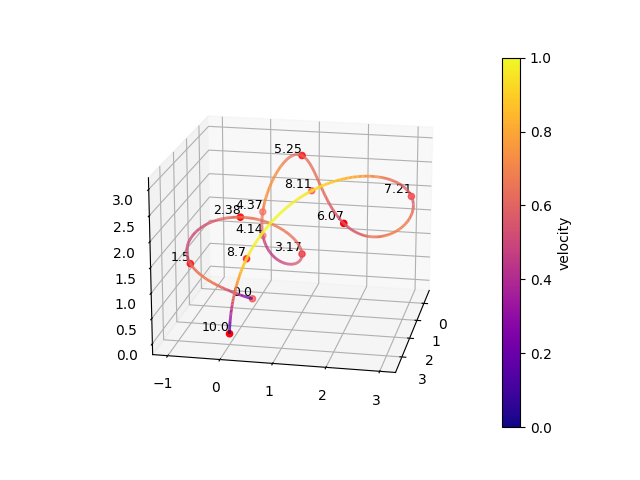
\includegraphics[width=0.6\textwidth]{images/figure3d.png}
  \caption[Primer trajektorije.]{Primer optimalne trajektorije glede na trzaj (3. odvod) in s končnim časom 10 s, kjer so z rdečimi pikami podane vmesne točke, ob njih pa so pripisani pripadajoči vmesni časi.}
  \label{fig:primer_trajektorije}
\end{figure}
% 3. luknja v raziskovanju
% 4. contributions
Doprinosi tega magistrskega dela so sledeči:
\begin{itemize}
    \item razvijemo metodo računanja drugih parcialnih odvodov optimalne rešitve spodnjega nivoja dvonivojskega optimizacijskega problema, kar nam omogoči uporabo Newtonove metode za optimizacijo zgornjega nivoja;

    \item izkoristimo bločno strukturo matrik cenovne funkcije in linearnih omejitev ter njunih odvodov, da dosežemo dodatne pohitritve;
    
    \item z eksperimenti pokažemo, da metoda skonvergira k lokalno optimalni rešitvi v povprečju v 10 korakih ne glede na stopnjo polinomov, optimizirane vrednosti ali števila segmentov;

    \item nadalje ugotovimo, da je Hessova matrika skoraj pasovna in da pri izračunu zgolj nekaj pasov Hessove matrike dosežemo pohitritev metode, pri čemer je vpliv izgube izvenpasovnih elementov Hessove matrike na konvergenco zanemarljiv;
    
    \item metoda je primerljivo hitra v primerjavi z obstoječimi rešitvami in ima potencial za nadaljne pohitritve s paralelizacijo na grafičnih procesnih enotah.
\end{itemize}
% 5. opis preostanka magistrske

Preostanek tega magistrskega dela je strukturiran na sledeči način. Najprej v poglavju~\ref{sec:pregled_podrocja} opišemo sorodna dela ter dela in pojme, ki služijo kot temelj naši metodi. Nato v poglavju~\ref{sec:opis_metode} predstavimo optimizacijski problem in podrobno opišemo našo metodo reševanja in jo teoretično podkrepimo. V poglavju~\ref{sec:eksperimenti} analiziramo implementacijo naše metode v smislu konvergence in hitrosti v odvisnosti od vhodnih parametrov. V poglavju~\ref{sec:zakljucek} povzamemo vsebino in predlagamo izboljšave in nadaljne delo.



\section{Pregled področja}
\label{sec:pregled_podrocja}

V tem poglavju opišemo sorodna dela in predstavimo pojme in dognanja, na katerih je naše delo osnovano. Najprej podamo opis diferencialno ploščatih sistemov in njihovo povezavo z optimizacijo trajektorij. Nato predstavimo trenutno stanje področja optimizacije trajektorij za kvadrotorje in raziskave, na katerih naše delo bodisi temelji, bodisi predstvaljajo alternativne pristope k reševanju podobnih problemov. Potem opišemo področje dvonivojske optimizacije, na koncu pa še Newtonovo metodo za iskanje ekstremov.

\subsection{Diferencialno ploščati sistemi}
V tem delu se opiramo na pojem diferencialne ploščatosti. Sistem upravljanja
\begin{equation}
    \dot{x} = f(x, u), \quad x \in \mathbb{R}^n, u \in \mathbb{R}^m
\end{equation}
je diferencialno ploščat, če lahko najdemo tak nabor izhodnih spremenljivk $y \in \mathbb{R}^m$ (ploščati izhodi), da lahko stanje $x$ in krmilni vhod $u$ izrazimo kot funkciji ploščatih izhodov in njihovih odvodov \cite{murray1995differential}:
\begin{align}
    x &= \phi(y, \dot{y}, \ddot{y}, \dots, y^{(p)}) \\
    u &= \psi(y, \dot{y}, \ddot{y}, \dots, y^{(q)}).
\end{align}

Diferencialno ploščati sistemi upravljanja so koristni v primerih, kot je naš, kjer želimo eksplicitno določiti trajektorije. Tako lahko iz dovolj gladke trajektorije (izhoda) preprosto zračunamo vhod in stanje sistema. Izkaže se, da so tudi kvadrotorji diferencialno ploščati sistemi; postopek prevedbe iz izhodov na vhode sistema kvadrotorja je opisan v \cite{mellinger2011minimum}. V tem delu se osredotočimo na generiranje optimalnih trajektorij, diferencialna ploščatost pa je pomembna, ker želimo, da sistem trajektoriji dejansko sledi.

\subsection{Optimizacija trajektorij brezpilotnikov}
Načrtovanje trajektorij brezpilotnikov s polinomskimi zlepki se je uveljavilo v \cite{mellinger2011minimum}, kjer so problem s fiksno razporeditvijo časa po segmentih definirali kot QP. Kasneje so v \cite{richter2016polynomial} izboljšali numerično stabilnost te metode tako, da so enakostne omejitve vključili v cenovno funkcijo, v \cite{burke2020generating} pa so se osredotočili na pohitritev in pokazali linearno časovno zahtevnost v odvisnosti od števila segmentov. V \cite{mellinger2011minimum} so predstavili tudi problem, kjer optimizirajo časovno razporeditev po segmentih; optimizacijo izvedejo z gradientnim spustom, kjer pa gradient izračunajo z metodo končnih diferenc, ki pa za izračun gradienta zahteva linearno mnogo rešitev QP v razmerju s številom segmentov. Ta problem rešijo v \cite{sun2021fast}, kjer gradient izračunajo analitično z občutljivostno analizo KKT pogojev QP. V \cite{gao2018online} čase segmentov določijo hevristično. V \cite{wang2021generating} problem s fiksnimi časi segmentov rešijo z dvojnim opisovanjem polinomov in dosežejo izjemne pohitritve.

Obstajajo tudi pristopi, ki ne ločijo časovnih in prostorskih spremenljivk \cite{zhou2020ego, fridovich2018planning} in se zanašajo na kompleksne algoritme za nelinearno programiranje \cite{wachter2006implementation}. Ti algoritmi pogosto omogočajo sočasno optimizacijo vmesnih točk znotraj določenega dopustnega območja, kar poveča prilagodljivost trajektorije.

\subsection{Dvonivojska optimizacija}
Dvonivojska optimizacija se ukvarja z optimizacijskimi problemi, kjer je cenovna funkcija enega optimizacijskega problema (zgornji nivo) odvisna od optimalne vrednosti odločitvenih spremenljivk drugega optimizacijskega problema (spodnji nivo). Splošna oblika dvonivojskega optimizacijskega problema je predstavljena kot:
\begin{equation}
    \begin{aligned}
        \min_{x\in X, y^*\in Y}& \quad F(x,y^*) \\
        \text{p.p.} & \quad y^* = \arg \min_{y\in Y} \{f(y) : g(x,y) \leq 0\} \\
        &\quad G(x,y^*) \leq 0
    \end{aligned}
\end{equation}

Znan primer dvonivojske optimizacije je Stacklebergova igra \cite{stackelberg1934marktform}, ki je igra med dvema igralcema (voditelj in sledilec), kjer voditelj optimizira svojo strategijo glede na sledilčevo. 

Dvonivojska optimizacija v načrtovanju trajektorij brezpilotnikov in v robotiki na splošno se navadno uporablja, ko je optimizacijski problem odvisen od časovne razporeditve in nekaterih drugih parametrov, ki pa so tudi odvisni od časovne razporeditve. V našem primeru so to koeficienti polinomov. Pogosto se, kot v našem primeru, izkaže, da se da spodnji nivo izraziti kot QP, ki se ga da rešiti s standardnimi knjižnicami. Tudi problem v \cite{mellinger2011minimum} je implicitno definiran kot dvonivojski optimizacijski problem. V \cite{sun2021fast} poleg izračuna analitičnih gradientov svojo rešitev podkrepijo teoretično. Izven domene načrtovanja trajektorij v \cite{amos2017optnet} dvonivojsko optimizacijo na QP uporabijo za integracijo QP kot plast v golobkih nevronskih mrežah, kjer so parametri QP odvisni od drugih plasti v nevronski mreži. V \cite{dyro2022second} razvijejo teorijo računanja Hessove matrike zgornjega problema splošnih dvonivojskih neomejenih optimizacijskih problemov z uporabo izreka of implicitni funkciji (IIF); z eksperimenti tudi pokažejo hitrejšo konvergenco kot obstoječe metode.

\subsection{Newtonova metoda}
Newtonova metoda je iterativna metoda za iskanje ekstremov dvakrat zvezno odvedljivih funkcij \cite{newton1736method, boyd2004convex}. Korak v iteraciji Newtonove metode za funkcije več spremenljivk se izračuna z enačbo

\begin{equation}
    x_{k+1} = x_k - [\nabla^2_f(x_k)]^{-1} \nabla_f(x_k), 
\end{equation}
kjer je $f : \mathbb{R}^n \to \mathbb{R}$ dvakrat zvezno odvedljiva funkcija, $x_k \in \mathbb{R}^n$ trenutna točka, $x_{k+1} \in \mathbb{R}^n$ pa naslednja točka iteracije. $\nabla^2_f(x_k)$ predstvavlja Hessovo matriko funkcije $f$ v točki $x_k$, $\nabla_f(x_k)$ pa gradient funkcije $f$ v točki $x_k$. Kot že omenjeno, v \cite{dyro2022second} razvijejo teorijo računanja gradienta in Hessove matrike za neomejene dvonivojske optimizacijske probleme in pokažejo hitro konvergenco. Tudi v tem delu eksperimenti pokažejo zelo hitro konvergenco k optimalni rešitvi.

\section{Opis metode}
\label{sec:opis_metode}

V tem poglavju opišemo našo metodo. Najprej definiramo osnovni problem v obliki minimizacije funkcionala z omejitvami s fiksnimi potovalnimi časi po segmentih. Nato pokažemo, kako se problem minimizacije funkcionala prevede na QP, kjer optimizacijske spremenljivke postanejo koeficienti polinomov. Dodamo optimizacijo po časih segmentov in predstavimo glavni optimizacijski problem, ki ga v tem delu rešujemo. Nato opišemo, kako lahko s pomočjo KKT pogojev QP izluščimo gradient in Hessovo matriko cenovne funkcije v zgornjem nivoju dvonivojskega problema. Zatem predstavimo minimizacijski algoritem, ki sloni na Newtonovi metodi. Na koncu pokažemo, kako lahko z uporabo bločne strukture matrik in strukture Hessove matrike dosežemo velike pohitritve. 

Najprej pa uvedemo nekaj nestandardne notacije, ki bo služila za boljšo preglednost in razumljivost v enačbah v tem poglavju:

Naj bo $\mathbf{A}(\mathbf{t}) \in \mathcal{C}^2(\mathbb{R}^k, \mathbb{R}^{m\times n})$ matrika, kjer je vsak element dvakrat zvezno odvedljiva funkcija vektorja $\mathbf{t}$.
\begin{itemize}
    \item S simbolom $\partial_{t_i} \mathbf{A}$ označimo matriko parcialnih odvodov glede na $i$-to komponento vektorja $\mathbf{t}$:
    \begin{equation} \partial_{t_i} \mathbf{A} := \frac{\partial \mathbf{A}(\mathbf{t})}{\partial t_i} = \left[ \frac{\partial a_{uv}(\mathbf{t})}{\partial t_i} \right]_{u,v=1}^{m,n} \end{equation}
    \item V nadaljevanju bomo zaradi večje preglednosti izpeljav pogosto opuščali eksplicitno navajanje argumenta $\mathbf{t}$ (npr. $\mathbf{A}$ namesto $\mathbf{A}(\mathbf{t})$), razen v primerih, ko je to nujno za razumevanje.
\end{itemize}


\subsection{Problem s podanimi časi segmentov}
Rešujemo spodnji problem:

Definirano imamo zaporedje vmesnih točk $P_0, \ldots P_n$ in potovalne čase za posamezen segment $t_1, \ldots, t_n$. Najti moramo polinome $p_1, \ldots, p_n$, ki minimizirajo spodnji funkcional:

\begin{equation}
\label{eq:functional}
\begin{aligned}
    \min_{p_1, \ldots p_n}& \quad \sum_{i=1}^n \int_0^{t_i} (p_i^{(r)}(\tau))^2 d\tau \\
    \text{p.p.} & \quad p_1(0) = P_0, \quad p_n(t_n) = P_n& \\
    & \quad p^{(k)}_1(0) = 0 \quad ; \quad &k = 1, \ldots, K \\
     &\quad p^{(k)}_n(t_n) = 0 \quad ; \quad &k = 1, \ldots, K \\
     \quad &p_i(t_i) = p_{i+1}(0) = P_i \quad ;& \quad i = 1, \ldots , n-1 \\
     \quad &p_i^{(k)}(t_i) = p_{i+1}^{(k)}(0) \quad ; \quad &i = 1, \ldots, n-1,\quad k = 1, \ldots, K 
\end{aligned}
\end{equation}
Pravzaprav tak problem rešujemo trikrat, posebej za vsako od osi $x$, $y$ ter $z$, kjer $t_i$ ostane isti, spremenijo pa se zgolj koordinate vmesnih točk $P_i$ za posamezno os. Z nekaj svobode pa lahko izberemo parametre:
\begin{itemize}
    \item $d$, stopnja polinomskih zlepkov
    \item $k$, red zveznosti trajektorije
    \item $r$, optimizacijska stopnja odvoda
\end{itemize}
Veljati mora $r \leq k \leq d$, standardne vrednosti pa so $d = 9$, $r = 3$ (trzaj) ali $r = 4$ (pok) ter $k = r$.

\subsection{Prevedba na QP}
V tem razdelku opišemo, kako problem, predstavljen v ~\eqref{eq:functional} prevedemo na QP oblike:
\begin{equation}
    \begin{aligned}
        &\frac{1}{2}\mathbf{a}^\top \mathbf{Q} \mathbf{a}\\
        \text{p.p.}\quad & \mathbf{A}\mathbf{a} = \mathbf{b},
    \end{aligned}
\end{equation}
kjer je $\mathbf{a} \in \mathbb{R}^{n (d+1)}$ optimizacijski vektor in predstavlja koeficiente polinomskih zlepkov, $\mathbf{Q} \in \mathbb{R}^{n(d+1) \times n(d+1)}$ je simetrična in pozitivno definitna matrika, $\mathbf{A} \in \mathbb{R}^{M \times n(d+1)}$ in $\mathbf{b} \in \mathbb{R}^M$ pa predstavljata linearne omejitve. Najprej bomo pokazali, kako izračunamo matriko $\mathbf{Q}$, nato pa še, kako izračunamo matriko $\mathbf{A}$ in vektor $\mathbf{b}$. Bistvenega pomena pri tej izpeljavi je, da so elementi matrik $\mathbf{Q}$ in $\mathbf{A}$ zvezno odvisni od vmesnih časov $t_i$.

\subsubsection{Izračun matrike $\mathbf{Q}$}
Matriko $\mathbf{Q}$ izračunamo tako, da ločeno prevedemo posamezen integral $\int_0^{t_i} (p_i^{(r)}(\tau))^2 d\tau$ na matrično enačbo $\mathbf{a}_i^\top \mathbf{Q}_i \mathbf{a}_i$, kjer je $\mathbf{a}_i$ vektor koeficientov $i$-tega polinoma. Celotno vsoto $\sum_{i=1}^n \int_0^{t_i} (p_i^{(r)}(\tau))^2 d\tau$ pa nato predstavimo kot bločno matriko
\begin{equation}
\label{eq:cost_function_matrix}
    \mathbf{a}^\top \mathbf{Q} \mathbf{a} = 
    \begin{bmatrix}
        \mathbf{a}_1 \\ \mathbf{a}_2 \\ \vdots \\ \mathbf{a}_n 
    \end{bmatrix}^\top
    \begin{bmatrix}
        \mathbf{Q}_1 & \mathbf{0} & \cdots & \mathbf{0} \\
        \mathbf{0} & \mathbf{Q}_2 & \cdots & \mathbf{0} \\
        \vdots & \vdots & \ddots & \vdots \\
        \mathbf{0} & \mathbf{0} & \cdots & \mathbf{Q}_n
    \end{bmatrix}
    \begin{bmatrix}
        \mathbf{a}_1 \\ \mathbf{a}_2 \\ \vdots \\ \mathbf{a}_n 
    \end{bmatrix}
\end{equation}

Če je 
\begin{equation}
    p(\tau) = \sum_{i = 0}^d a_{i} \tau^i,
\end{equation}

potem velja:
\begin{equation}
    p^{(k)}(\tau) = \sum_{i = k}^d [\prod_{m=0}^{k-1} (i-m)]a_{i} \tau^{i-r},
\end{equation}

in

\begin{equation}
    p(t)^2 = \sum_{i=0}^{2N} \left( \sum_{j=0}^{i} p_j p_{i-j} \right) t^i
\end{equation}

\begin{equation}
    (p^{(k)}(\tau))^2 = \sum_{i=2r}^{2N} \left( \sum_{j=r}^{i-r} a_j a_{i-j} \prod_{m=0}^{r-1} (j - m)(i - j - m) \right) \tau^{i-2r}
\end{equation}

\begin{equation}
\int_{0}^t (p^{(k)}(\tau))^2d\tau = \sum_{i=0}^{2N} \left( \sum_{j=r}^{N} \prod_{m=0}^{r-1} (j - m)(i - j - m) a_j a_{i-j} \right) \frac{t^{i-2r+1}}{i - 2r + 1}
\end{equation}

Sedaj že lahko vidimo, da ima izraz obliko:
\begin{equation}
    \int_{0}^t (p^{(k)}(\tau))^2d\tau = \sum_{k=0}^N\sum_{l=0}^N a_ka_l \mathbf{Q}_{kl} = \mathbf{a}^\top \mathbf{Q} \mathbf{a}
\end{equation}
za neko matriko $\mathbf{Q}$. Elemente $\mathbf{Q}_{kl}$ pa izračunamo tako, da izračunamo 
\begin{equation}
    \mathbf{Q}_{kl} = \frac{\partial^2}{\partial a_k \partial a_l}  (a_ka_l\mathbf{Q}_{kl}) = \frac{\partial^2}{\partial a_k \partial a_l} \left( \sum_{i=0}^{2N} \left( \sum_{j=r}^{N} \prod_{m=0}^{r-1} (j - m)(i - j - m) a_j a_{i-j} \right) \frac{t^{i-2r+1}}{i - 2r + 1} \right)
\end{equation}

\subsubsection{Izračun matrike $\mathbf{A}$ in vektorja $\mathbf{b}$}

\subsection{Problem s časovnimi spremenljivkami}

\begin{figure}
     \centering
     \begin{subfigure}[b]{0.48\textwidth}
         \centering
         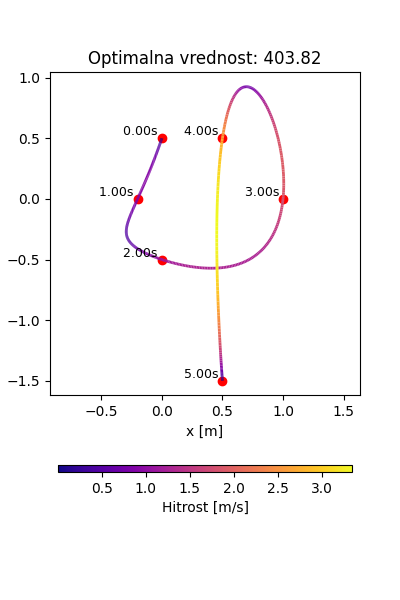
\includegraphics[width=\textwidth]{images/phi_fixed_time.png}
         \caption{Trajektorija s fiksno določenimi vmesnimi časi.}
         \label{fig:fixed_time}
     \end{subfigure}
     \hfill
     \begin{subfigure}[b]{0.48\textwidth}
         \centering
         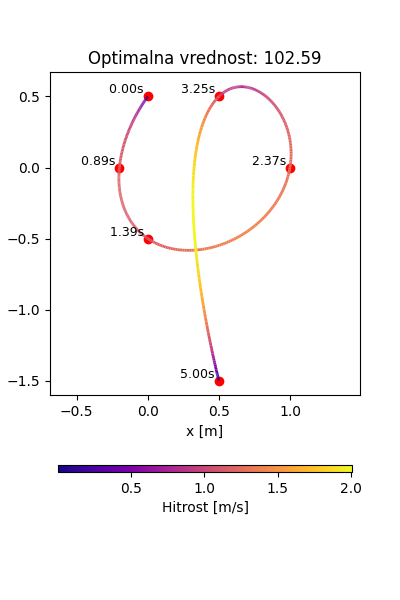
\includegraphics[width=\textwidth]{images/phi_variable_time.png}
         \caption{Trajektorija z optimiziranimi vmesnimi časi.}
         \label{fig:variable_time}
     \end{subfigure}
     \caption{Primerjava trajektorij, kjer fiksno določimo vmesne čase (a), in kjer izvedemo optimizacijo po vmesnih časih (b). Obe trajektoriji imata končni čas 5s, vendar ima desna trajektorija nižjo optimialno vrednost in tudi nižjo maksimalno hitrost.}
     \label{fig:primerjava_fixed_variable}
\end{figure}

V prejšnjem poglavju smo predstavili problem, kjer so časi segmentov podani kot fiksni parametri problema. Pogosto pa nam je pomemben le celoten čas potovanja po trajektoriji. Na primer, slika~\ref{fig:primerjava_fixed_variable} nudi primerjavo med fiksno določenimi vmesnimi časi in optimiziranimi vmesnimi časi za isto zaporedje vmesnih točk in isti skupen čas. Če nam je vseeno, kakšni so časi na vmesnih točkah, je očitno, da optimizacija časov segmentov vodi do bistveno boljše trajektorije. Zato lahko definiramo želen skupen čas trajektorije $T$ in vektor spremenljivk $\mathbf{t} = \left[ t_1, t_2, \ldots , t_n\right]$, kjer velja $\sum_{i=1}^n t_i = T$ in $t_i > 0$.  Sedaj lahko formuliramo nov optimizacijski problem:

\begin{equation}
    \begin{aligned}
        \min_{\mathbf{t},\mathbf{a}} & \quad \frac{1}{2}\mathbf{a}^\top \mathbf{Q}(\mathbf{t}) \mathbf{a}\\
        \text{p.p.} & \quad \mathbf{A}(\mathbf{t})\mathbf{a} = \mathbf{b}\\
        & \quad \mathbf{t} > \mathbf{0} \\
        & \quad \mathbf{1}^\top \mathbf{t} = T,
    \end{aligned}
\end{equation}
kjer je $\mathbf{1}$ vektor enic. Očitno je, da ta problem ni konveksen, niti nima konveksnih omejitev. Zato ga je koristno reformulirati v sledečo ekvivalentno dvonivojsko obliko:

\begin{equation}
    \begin{aligned}
        \min_{\mathbf{t},\mathbf{a^*}}& \quad F(\mathbf{t}) := \frac{1}{2}\mathbf{a^{*\top}}\mathbf{Q}(\mathbf{t})\mathbf{a^*} \\
        \text{p.p.}& \quad\mathbf{a^*} = \arg \min_\mathbf{a} \{\frac{1}{2}\mathbf{a}^\top\mathbf{Q}(\mathbf{t})\mathbf{a} : \mathbf{A}(\mathbf{t})\mathbf{a} = \mathbf{b}\}\\
        & \quad \mathbf{t} > \mathbf{0} \\
        & \quad \mathbf{1}^\top \mathbf{t} = T,
    \end{aligned}
\end{equation}

kjer problemu računanja $\mathbf{a}^*$ rečemo spodnji nivo dvonivojskega optimizacijskega problema, problemu minimizacije $F(\mathbf{t})$ pa zgornji nivo. Če fiksiramo $\mathbf{t}$, je spodnji nivo preprost QP z enakostnimi omejitvami. S takim problemom se srečujejo v \cite{mellinger2011minimum, sun2021fast}, kjer v neki točki $\mathbf{t}'$ izračunajo gradient $\nabla_\mathbf{t}F(\mathbf{t}')$ in izvedejo gradientni spust. Pri tem za izračun gradienta v \cite{mellinger2011minimum} uporabijo metodo končnih diferenc, v \cite{sun2021fast} pa ga izračunajo analitično.

To je glavni optimizacijski problem, s katerim se v tem magistrskem delu ukvarjamo in preostanek tega poglavja je posvečen opisu naše metode njegovega reševanja. V naslednjem podpoglavju bomo s pomočjo KKT pogojev in izreka o implicitni funkciji pokazali, da velja $\mathbf{a}^* \in \mathcal{C}^\infty(\mathbf{t})$ in kako izračunati parcialne odvode tega vektorja, kar nam bo omogočilo računanje analitičnih parcialnih odvodov višjega reda za $F(\mathbf{t})$ in s tem gradienta in Hessove matrike.

%Dodatno, $\mathbf{Q}, \mathbf{A} \in \mathcal{C}^{\infty}(\mathbb{R}^n)$.

\subsection{Odvajanje s KKT pogoji}

V tem podpoglavju bomo predstavili, kako s pomočjo KKT pogojev izračunamo gradient in Hessovo matriko cenovne funkcije zgornjenivojskega problema. Najprej predstavimo izrek o KKT pogojih za splošen optimizacijski program in opišemo lastnosti KKT pogojev, če imamo konveksen optimizacijski program. Nato v \ref{} definiramo KKT matriko za QP z enakostnimi omejitvami. V \ref{} navedemo izrek o implicitni funkciji in pokažemo, da je v resnici $\mathbf{a^*} = \mathbf{a^*}(\mathbf{t})$ analitična funkcija. S tem argumentiramo izračun parcialnih odvodov $\mathbf{a^*}$ ter gradienta in Hessove matrike, ki jih predstavimo v \ref{} in \ref{}.

Spodaj navedemo standarden izrek o KKT pogojih \cite{bertsekas1997nonlinear}.

\textbf{Karush-Kuhn-Tuckerjevi pogoji.} Za optimizacijski program
\[
\min_x f(x) \quad \text{p.p.} \quad g_i(x) \leq 0, \ i=1,\dots,m, \quad h_j(x) = 0, \ j=1,\dots,p,
\]
so Karush-Kuhn-Tuckerjevi pogoji naslednji: obstajajo Lagrangeevi multiplikatorji $\lambda \in \mathbb{R}^m_{\geq 0}$, $\mu \in \mathbb{R}^p$, da velja
\begin{align}
\nabla f(x) + \sum_{i=1}^m \lambda_i \nabla g_i(x) + \sum_{j=1}^p \mu_j \nabla h_j(x) &= 0, \label{eq:kkt-stationarity} \\
\lambda_i g_i(x) &= 0, \quad i=1,\dots,m, \label{eq:kkt-complementarity} \\
g_i(x) &\leq 0, \quad i=1,\dots,m, \label{eq:kkt-primal-feasibility} \\
h_j(x) &= 0, \quad j=1,\dots,p, \label{eq:kkt-equality} \\
\lambda &\geq 0. \label{eq:kkt-dual-feasibility}
\end{align}

Za \emph{konveksne programe}, kjer je $f$ konveksna, $g_i$ konveksne, $h_j$ afine in velja Slaterjev pogoj, postanejo KKT pogoji \emph{potrebni in zadostni} za globalno optimalnost. Slaterjev pogoj predstavimo spodaj.

\textbf{Slaterjev pogoj \cite{bertsekas1997nonlinear,boyd2004convex}.} 
Za konveksni program
\[
\min_x f(x) \quad \text{p.p.} \quad g_i(x) \leq 0, \ i=1,\dots,m, \quad h_j(x) = 0, \ j=1,\dots,p,
\]
Slaterjev pogoj velja, če obstaja $x^\circ$ tako, da
\begin{itemize}
\item $g_i(x^\circ) < 0$ za vse $i=1,\dots,m$ (stroga neenakostna dopustnost),
\item $h_j(x^\circ) = 0$ for all $j=1,\dots,p$ (enakostna dopustnost).
\end{itemize}

Opazimo lahko, da v primeru, kjer neenakostnih omejitem ni, Slaterjev pogoj velja.

\subsubsection{KKT pogoji QP}

V primeru našega optimizacijskega problema, kjer imamo kvadratično cenovno funkcijo in enakostne omejitve, lahko privzamemo Slaterjev pogoj, saj nimamo neenakostnih omejitev, KKT pogoji pa se zreducirajo na:

\begin{equation}
    \begin{aligned}
        \nabla (\frac{1}{2}\mathbf{a^{*\top}}\mathbf{Q}\mathbf{a^*}) + \sum_{i=1}^m \mathbf{\mu^*}_i \nabla(\mathbf{A}_i \mathbf{a^*}) = \mathbf{0}& \\
        \mathbf{A}_i \mathbf{a^*} - \mathbf{b}_i = 0&, \quad i = 1,\ldots, m.
    \end{aligned}
\end{equation}

\begin{equation}
    \begin{aligned}
        \mathbf{Q}\mathbf{a^*} + \mathbf{A^\top}\mathbf{\mu^*} = \mathbf{0}& \\
        \mathbf{A} \mathbf{a^*} = \mathbf{b}&
    \end{aligned}
\end{equation}

Pri optimalnosti velja naslednja matrična enačba, kjer so $\mathbf{\mu}$ enakostni Lagrangeevi multiplikatorji, $\mathbf{a^*}$, ter $\mathbf{\mu^*}$ pa so vrednosti $\mathbf{a}$ ter $\mathbf{\mu}$ pri optimalnosti:
\begin{equation}
    \begin{gathered}
        % Top Equation
        \underbrace{
            \begin{bmatrix}
                \qmat & \amat^{\top} \\
                \amat & \mathbf{0}
            \end{bmatrix}
        }_{\kmat}
        \underbrace{
            \begin{bmatrix}
                \avec^* \\
                \boldsymbol{\mu}^*
            \end{bmatrix}
        }_{\mathbf{y}^*}
        -
        \underbrace{
            \begin{bmatrix}
                \mathbf{0} \\
                \bvec
            \end{bmatrix}
        }_{\mathbf{c}}
        = \mathbf{0}
    \end{gathered}
\end{equation}


V nadaljevanju bomo izmenično uporabljali tako osnovno kot kompaktno obliko ($\kmat \mathbf{y}^* - \matnbf{c} = \mathbf{0}$) zapisa KKT pogojev. Kompaktno obliko bomo uporabili, kjer bo to pripomoglo k boljši preglednosti, osnovno obliko pa tam, kjer bo pomembna struktura posameznih delov matrike $\kmat$, ali pa bo treba ločiti med primarnimi in dualnimi komponentami $\mathbf{y}^*$.

\subsubsection{Izrek o implicitni funkciji}
\label{sec:ift}

Z uporabo izreka o implicitni fukciji lahko pokažemo, da obstaja odprta množica $U$ in gladke funkcije $\yimplicit$ : $U \to \R^{m+n}$, $\aimplicit$ : $U \to \R^{n}$, $\muimplicit$ : $U \to \R^{m}$, kjer velja $\yimplicit(\tvec) = (\aimplicit(\tvec), \muimplicit(\tvec)) = (\avec^*, \muvec^*)$. To nam da formalno podlago, da cenovno funkcijo $F(\tvec)$ odvajamo glede na $\tvec$, saj jo lahko zapišemo kot:

\begin{equation}
    F(\mathbf{t}) = \frac{1}{2}\avec^{*\top}\qmat(\tvec)\avec^* = \frac{1}{2} \aimplicit(\tvec)^\top \qmat(\tvec) \aimplicit(\tvec)
\end{equation}

Dodatno velja:
\begin{equation}
    \label{eq:equilibrium_implicit}
    \kmat(\tvec) \mathbf(y)^* - \mathbf{c} = \kmat(\tvec) \yimplicit(\tvec) - \mathbf{c} = \mathbf{0}
\end{equation}

V tem razdelku najprej podamo izrek o implicitni funkciji \cite{rudin1976principles} in nato pokažemo, kako z njim argumentiramo obstoj gladkih funkcij $\yimplicit$, $\aimplicit$ in $\muimplicit$.

\begin{izrek}[Izrek o implicitni funkciji]
    Naj bo $f: \mathbb{R}^{m+n} \to \mathbb{R}^m$ zvezno odvedljiva funkcija in naj ima $\mathbb{R}^{m+n}$ koordinate $(\mathbf{x},\mathbf{y})$. 
    
    Fiksirajmo točko $(\mathbf{a}, \mathbf{b}) = (a_1, a_2, \ldots, a_m, b_1, b_2, \ldots, a_n)$, kjer velja $f(\mathbf{a},\mathbf{b}) = \mathbf{0}$ in $\mathbf{0} \in \mathbb{R}^m$ je ničelni vektor. Če je Jacobijeva matrika:
    \begin{equation}
        J_{f,\mathbf{y}}(\mathbf{a}, \mathbf{b}) = \left[ \frac{\partial f_i}{\partial y_j} (\mathbf{a},\mathbf{b})\right]
    \end{equation}

    obrnljiva, potem obstaja odprta množica $U \in \mathbb{R}^n$, ki vsebuje $\mathbf{a}$, tako da obstaja enolična funkcija $g:U \to \mathbb{R}^m$, kjer $g(\mathbf{a}) = \mathbf{b}$ in $f(\mathbf{x}, g(\mathbf{x})) = \mathbf{0}$ za vse $\mathbf{x} \in U$. Nadalje, $g$ je zvezno odvedljiva in Jacobijeva matrika parcialnih odvodov $g$ v $U$ je definirana kot:
    \begin{equation}
        \left[\frac{\partial g_i}{\partial x_j}(\mathbf{x})\right]_{m \times n}
= -\left[ J_{f, \mathbf{y}}(\mathbf{x}, g(\mathbf{x})) \right]^{-1}_{m \times m}
\left[ J_{f,\mathbf{x}}(\mathbf{x}, g(\mathbf{x})) \right]_{m \times n}
    \end{equation}, kjer je 

\begin{equation}
        J_{f,\mathbf{x}}(\mathbf{a}, \mathbf{b}) = \left[ \frac{\partial f_i}{\partial x_j} (\mathbf{a},\mathbf{b})\right]
    \end{equation}
\end{izrek}

\begin{izrek} [Gladkost rešitve KKT pogojev]
Naj velja enačba $K\mathbf{y}^* - \mathbf{c} = \mathbf{0}$, kjer je $\mathbf{y}^* = (\mathbf{a}^*, \mathbf{\mu}^*)$ rešitev KKT pogojev QP z enakostnimi omejitvami. Potem obstaja odprta množica $U \subset \mathbb{R}^n$ in gladke funkcije $\yimplicit : U \to \mathbb{R}^{m+n}$, $\aimplicit : U \to \mathbb{R}^{n}$, $\muimplicit : U \to \mathbb{R}^{m}$, kjer velja $\yimplicit(\tvec) = (\aimplicit(\tvec), \muimplicit(\tvec)) = (\avec^*, \muvec^*)$.
\end{izrek}

\begin{dokaz}
Pokazati moramo, da je Jacobijeva matrika parcialnih odvodov enačbe $K\mathbf{y}^* - \mathbf{c}$ glede na $\mathbf{y}^*$ obrnljiva. Ni težko videti, da je Jacobijeva matrika parcialnih odvodov kar KKT matrika $\mathbf{K}$. Ker je $\mathbf{Q}$ pozitivno definitna in ker ima $\mathbf{A}$ poln rang, je matrika $\mathbf{K}$ obrnljiva \cite{EPFL_Part5}. S tem je pogoj izreka o implicitni funkciji izpolnjen in sledi obstoj gladkih funkcij $\yimplicit$, $\aimplicit$ in $\muimplicit$.
\end{dokaz}

\subsubsection{Računanje gradienta}

V tem razdelku predstavimo, kako izračunamo gradient cenovne funkcije $F(\tvec)$. Začnemo z zapisom parcialnega odvoda $F(\tvec)$ glede na komponento $t_i$:
\begin{equation}
    \partial_{t_i} F(\tvec) = \frac{1}{2} \left( \partial_{t_i} \aimplicit(\tvec)^\top \qmat(\tvec) \aimplicit(\tvec) + \aimplicit(\tvec)^\top \partial_{t_i} \qmat(\tvec) \aimplicit(\tvec) + \aimplicit(\tvec)^\top \qmat(\tvec) \partial_{t_i} \aimplicit(\tvec) \right)
\end{equation}

Iz enačbe~\eqref{eq:equilibrium_implicit} lahko izrazimo parcialni odvod $\partial_{t_i} \yimplicit(\tvec)$ kot:
\begin{equation}
    \begin{aligned}
        \kmat \yimplicit(\tvec) - \mathbf{c} &= \mathbf{0} \\
        \partial_{t_i}(\kmat \yimplicit(\tvec) - \mathbf{c}) &= \mathbf{0} \\
        \partial_{t_i}\kmat \yimplicit(\tvec) + \kmat \partial_{t_i} \yimplicit(\tvec) &= \mathbf{0} \\
        \kmat \partial_{t_i} \yimplicit(\tvec) &= - \partial_{t_i}\kmat \yimplicit(\tvec)
    \end{aligned}
\end{equation}

Ker je matrika $\kmat$ obrnljiva, bi lahko paricalni odvod $\partial_{t_i} \yimplicit(\tvec)$ izračunali eksplicitno, vendar v naši rešitvi inverza $\kmat^{-1}$ zaradi boljše časovne učinkovitosti pravzaprav nikoli ne izračunamo, vendar rešujemo sisteme enačb s to matriko.

Iz $\partial_{t_i} \yimplicit(\tvec)$ lahko sedaj vzamemo komponento $\partial_{t_i} \aimplicit(\tvec)$ in jo vstavimo v izraz za $\partial_{t_i} F(\tvec)$.

\subsubsection{Računanje Hessove matrike}

\subsection{Newtonova metoda in optimizacijski algoritem}

\begin{algorithm}
\caption{Linijsko iskanje z vračanjem (Backtracking Line Search)}
\label{alg:backtracking}
\begin{algorithmic}[1]
\REQUIRE Trenutna točka $\mathbf{t}_k$, smer $\Delta \mathbf{t}_k$, gradient $\nabla F(\mathbf{t}_k)$
\ENSURE Korak $\gamma$, ki zadošča Armijovemu pogoju
\STATE Nastavi parametra: $\alpha \in (0, 0.5)$ (npr. $0.01$), $\beta \in (0, 1)$ (npr. $0.5$)
\STATE $\gamma \leftarrow 1$
\WHILE{$F(\mathbf{t}_k + \gamma \Delta \mathbf{t}_k) > F(\mathbf{t}_k) + \alpha \gamma \nabla F(\mathbf{t}_k)^\top \Delta \mathbf{t}_k$}
    \STATE $\gamma \leftarrow \beta \gamma$
    \IF{$\gamma < \epsilon$}
        \STATE \textbf{break} \COMMENT{Preprečimo numerične težave}
    \ENDIF
\ENDWHILE
\RETURN $\gamma$
\end{algorithmic}
\end{algorithm}

\subsection{Pohitritve}

\section{Eksperimenti}
\label{sec:eksperimenti}

\subsection{Implementacija in uporaba zunanjih knjižnic}
Naša metoda je implementirana v programskem jeziku Python in je dostopna na povezavi \href{https://github.com/maticpokorn/trajectory_optimization}{\texttt{github.com/maticpokorn/trajectory\_optimization}}. V implementaciji se često zanašamo na operacije z redkimi matrikami za doseganje višje hitrosti in zato uprabljamo modul \texttt{scipy.sparse} knjižnice SciPy \cite{2020SciPy-NMeth}. Konkretno se poslužujemo metode SuperLU za faktorizacijo matrike~\eqref{} \cite{superlu1997superlu}. Za reševanje QP uporabljamo knjižnico OSQP \cite{osqp}. Implemetacijo naše metode sta omogočili še knjižnici NumPy \cite{harris2020array} in Matplotlib \cite{Hunter:2007}.

\subsection{Konvergenca}

\subsection{Hitrost}

\subsection{Pasovna struktura Hessove matrike}

\section{Zaključek}
\label{sec:zakljucek}

Ostaja mnogo poti za izboljšavo. Glavni izmed njih je vključitev neenakostnih omejitev v QP, kar bi omogočilo načrtovanje trajektorij z izogibanjem preprekam in omejitev maksimalnih hitrosti in pospeškov kvadrotorjev. Nadalje, implementacija v nižjenivojskem jeziku, kot je C++, bi z veliko verjetnostjo bistveno izboljšala hitrost. Uporaba metode ničelnega prostora za faktorizacijo matrike v enačbi~\eqref{} \cite{rees2014null} bi lahko pripomogla k dodatni pohitritvi.

\section{Integrali po \texorpdfstring{$\omega$}{ω}-kompleksih}
\subsection{Definicija}
\begin{definicija}
  Neskončno zaporedje kompleksnih števil, označeno z $\omega = (\omega_1, \omega_2, \ldots)$,
  se imenuje \emph{$\omega$-kompleks}.\footnote{To ime je izmišljeno.}

  Črni blok zgoraj je tam namenoma. Označuje, da \LaTeX{} ni znal vrstice prelomiti pravilno
  in vas na to opozarja. Preoblikujte stavek ali mu pomagajte deliti problematično besedo z
  ukazom \verb|\hyphenation{an-ti-ko-mu-ta-ti-ven}| v preambuli.
\end{definicija}
\begin{trditev}[Znano ime ali avtor]
  \label{trd:obstoj-omega}
  Obstaja vsaj en $\omega$-kompleks.
\end{trditev}
\begin{proof}
  Naštejmo nekaj primerov:
  \begin{align}
    \omega &= (0, 0, 0, \dots), \label{eq:zero-kompleks} \\
    \omega &= (1, i, -1, -i, 1, \ldots), \nonumber \\
    \omega &= (0, 1, 2, 3, \ldots). \nonumber \qedhere  % postavi QED na zadnjo vrstico enačbe
  \end{align}
\end{proof}

\section{Tehnični napotki za pisanje}

%\subsection{Sklicevanje in citiranje}
%Za sklice uporabljamo \verb|\ref|, za sklice na enačbe \verb|\eqref|, za citate \verb|\cite|. Pri
%sklicevanju in citiranju sklicano številko povežemo s prejšnjo besedo z nedeljivim presledkom
%$\sim$, kot npr.\ \verb|iz trditve~\ref{trd:obstoj-omega} vidimo|.

%\begin{primer}
%  Zaporedje~\eqref{eq:zero-kompleks} iz dokaza trditve~\ref{trd:obstoj-omega} na
%  strani~\pageref{trd:obstoj-omega} lahko najdemo tudi v Spletni enciklopediji zaporedij~\cite{oeis}.
%  Citiramo lahko tudi bolj natančno~\cite[trditev 2.1, str.\ 23]{lebedev2009introduction}.
%\end{primer}

\subsection{Okrajšave}
Pri uporabi okrajšav \LaTeX{} za piko vstavi predolg presledek, kot npr. tukaj. Zato se za vsako
piko, ki ni konec stavka doda presledek običajne širine z ukazom \verb*|\ |, kot npr.\ tukaj.
Primerjaj z okrajšavo zgoraj za razliko.

\subsection{Vstavljanje slik}
Sliko vstavimo v plavajočem okolju \texttt{figure}. Plavajoča okolja \emph{plavajo} po tekstu, in
jih lahko postavimo na vrh strani z opcijskim parametrom `\texttt{t}', na lokacijo, kjer je v kodi s
`\texttt{h}', in če to ne deluje, potem pa lahko rečete \LaTeX u, da ga \emph{res} želite tukaj,
kjer ste napisali, s `\texttt{h!}'. Lepo je da so vstavljene slike vektorske (recimo \texttt{.pdf}
ali \texttt{.eps} ali \texttt{.svg}) ali pa \texttt{.png} visoke resolucije (več kot
\unit[300]{dpi}).  Pod vsako sliko je napis in na vsako sliko se skličemo v besedilu. Primer
vektorske slike je na sliki~\ref{fig:sample}. Vektorsko sliko prepoznate tako, da močno
zoomate v sliko, in še vedno ostane gladka. Več informacij je na voljo na
\url{https://en.wikibooks.org/wiki/LaTeX/Floats,_Figures_and_Captions}. Če so slike bitne, kot na
primer slika~\ref{fig:image}, poskrbite, da so v dovolj visoki resoluciji.

\begin{figure}[h]
  \centering
  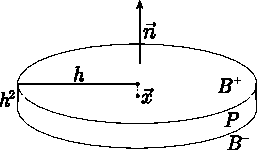
\includegraphics[width=0.6\textwidth]{images/sample.pdf}
% \caption[caption za v kazalo]{Dolg caption pod sliko}
  \caption[Primer vektorske slike.]{Primer vektorske slike z oznakami v enaki pisavi, kot jo
     uporablja \LaTeX{}.  Narejena je s programom Inkscape, \LaTeX{} oznake so importane v
     Inkscape iz pomožnega PDF.}
  \label{fig:sample}
\end{figure}

\begin{figure}[h]
  \centering
  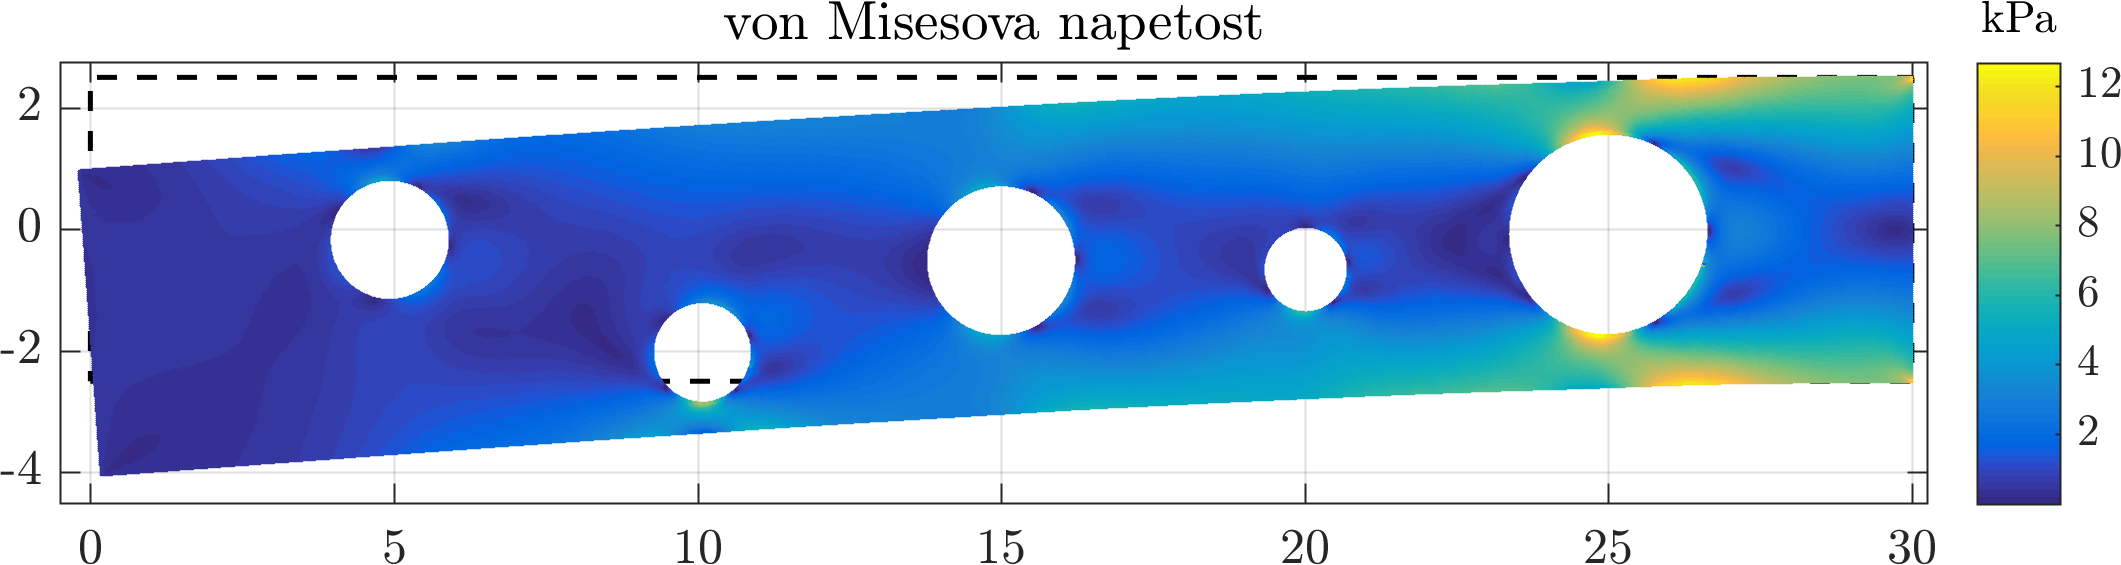
\includegraphics[width=0.8\textwidth]{images/image.png}
  \caption[Primer bitne slike.]{Primer bitne slike, izvožene iz Matlaba. Poskrbite, da so slike v
  dovolj visoki resoluciji in da ne vsebujejo prosojnih elementov (to zahteva PDF/A-1b format).}
  \label{fig:image}
\end{figure}

%\subsection{Kako narediti stvarno kazalo}
%Dodate ukaze \verb|\index{polje}| na besede, kjer je pojavijo, kot tukaj\index{tukaj}.
%Več o stvarnih kazalih je na voljo na \url{https://en.wikibooks.org/wiki/LaTeX/Indexing}.

%\subsection{Navajanje literature}
%Članke citiramo z uporabo \verb|\cite{label}|, \verb|\cite[text]{label}| ali pa več naenkrat s
%\verb|\cite\{label1, label2}|. Tudi tukaj predhodno besedo in citat povežemo z nedeljivim presledkom
%$\sim$. Na primer~\cite{chen2006meshless,liu2001point}, ali pa \cite{kibriya2007empirical}, ali pa
%\cite[str.\ 12]{trobec2015parallel}, \cite[enačba (2.3)]{pereira2016convergence}.
%Vnosi iz \verb|.bib| datoteke, ki niso citirani, se ne prikažejo v seznamu literature, zato jih
%tukaj citiram.~\cite{vene2000categorical}, \cite{gregoric2017stopniceni}, \cite{slak2015induktivni},
%\cite{nsphere}, \cite{kearsley1975linearly}, \cite{STtemplate}, \cite{NunbergerTand}, \cite{vanoosten2008realizability}.

\end{document}
